\documentclass[preprint]{revtex4-1}
\usepackage{graphicx}
\usepackage{epstopdf}
\usepackage{amsmath}
\usepackage{hyperref}
\usepackage{booktabs}
\usepackage{color}

\usepackage{SIunits}
\newcommand{\wstar}{-0.023}
\newcommand{\Qstar}{0.25}

\setlength{\tabcolsep}{10pt}

\newenvironment{sistema}%
  {\left\lbrace\begin{array}{@{}l@{}}}%
  {\end{array}\right.}


\usepackage{pgfplots}
\usepgfplotslibrary{external}
\usepgfplotslibrary{groupplots}
\usetikzlibrary{positioning}
\usetikzlibrary{plotmarks}
\tikzexternalize
\tikzset{external/force remake}
\tikzset{every mark/.append style={scale=0.8}}
\pgfplotsset{every axis/.append style={small}}

\begin{document}

\begin{figure}
	\centering
	\begin{tikzpicture}[
		pic3d/.style={inner sep=0}, %
		lab/.style={above right, text height=0.8em, text depth=0.2em, font=\bfseries}%
		]%
		\node[pic3d] (m3d) {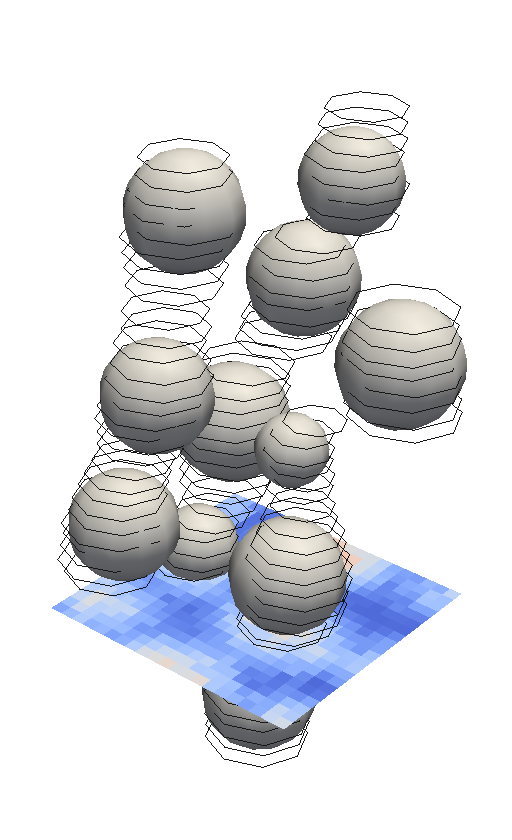
\includegraphics[width=0.28\textwidth]{comp2D3D_crop}};
		\node[lab] at (m3d.south west) {a};
		\node [pic3d, right] at (m3d.east) (m2d) {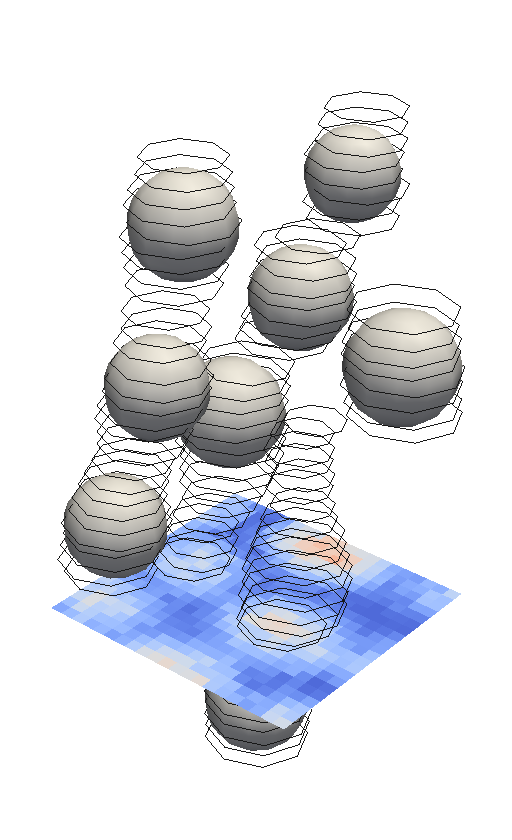
\includegraphics[width=0.28\textwidth]{comp2D_reconstructed_crop}};
		\node[lab] at (m2d.south west) {b};
		\node [pic3d, below right] at (m2d.north east) (cg20) {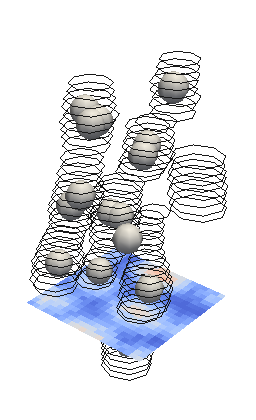
\includegraphics[width=0.14\textwidth]{comp3D_monoscale_r20_crop}};
		\node[lab] at (cg20.south west) {c};
		\node [pic3d, right] at (cg20.east) (cg25) {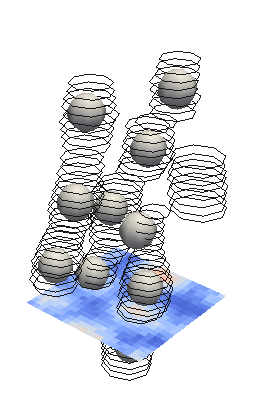
\includegraphics[width=0.14\textwidth]{comp3D_monoscale_r25_crop}};
		\node[lab] at (cg25.south west) {d};
		\node [pic3d, right] at (cg25.east) (cg30) {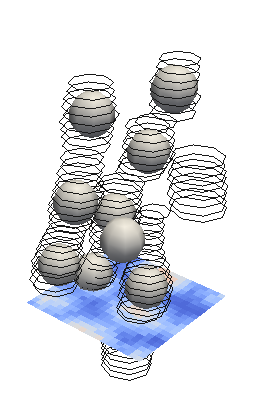
\includegraphics[width=0.14\textwidth]{comp3D_monoscale_r30_crop}};
		\node[lab] at (cg30.south west) {e};
		\node [pic3d, above right] at (m2d.south east) (cg35) {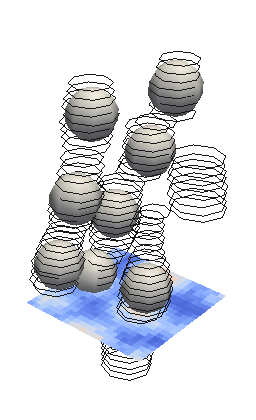
\includegraphics[width=0.14\textwidth]{comp3D_monoscale_r35_crop}};
		\node[lab] at (cg35.south west) {f};
		\node [pic3d, right] at (cg35.east) (cg40) {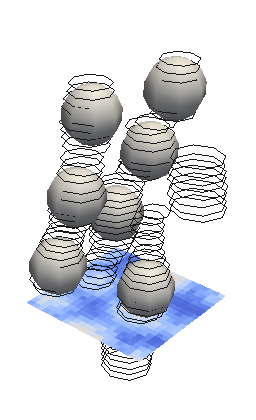
\includegraphics[width=0.14\textwidth]{comp3D_monoscale_r40_crop}};
		\node[lab] at (cg40.south west) {g};
		\node [pic3d, right] at (cg40.east) (cg45) {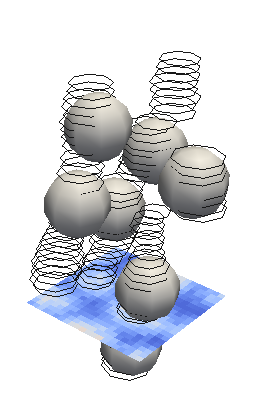
\includegraphics[width=0.14\textwidth]{comp3D_monoscale_r45_crop}};
		\node[lab] at (cg45.south west) {h};
	\end{tikzpicture}
	\caption{\textbf{Visualisation of the results of various tracking methods for the same portion of image.} \textbf{a} Multiscale 3D tracking. \textbf{b} Reconstruction from 2D tracking. \textbf{c-h} Crocker and Grier in 3D with blurring radius increasing from \unit{2}{px} to \unit{4.5}{px} by steps of \unit{0.5}{px}. The circles on each picture are the result of 2D multiscale tracking of each XY slice of the 3D pictures. Sphere are displayed with radii determined by the tracking methods in \textbf{a-b}, and equal to the blurring radius for \textbf{c-h}.}
	\label{fig:result3d}
\end{figure}


\end{document}